%------------------------------------------------------------------------------------------------------------

% Commands

\newcommand{\HEPfit}{{\tt HEPfit}}

%------------------------------------------------------------------------------------------------------------

\subsection{Global constraints on universal new physics at the HL/HE-LHC}
\begin{center}
	\textit{J. de Blas, M. Ciuchini, E. Franco, S. Mishima, M. Pierini, L. Reina and L. Silvestrini}
\end{center}

%%%%%%%%%%%%%%%%%%%%%%%%%%%%%%%%%%%%%%%%%%%%%%%%%%%%%

\subsubsection{Introduction}




%For concreteness, we will focus our analysis on the 
%so-called {\it universal theories}~\cite{Barbieri:2004qk,Wells:2015uba},
%which we briefly introduce in the next section.


%Our study is performed using the \HEPfit\, package. The 
%
%details on the parameters and procedure of the fit, including
%the extrapolations of HL/HE-LHC accuracies that have been used, are discussed
%in Section~\ref{sec:global-fit}.  We
%conclude by presenting results for the bounds obtained on the Wilson
%coefficients of the Lagrangian effective operators, both from a global
%fit when all operators are simultaneously active and from a fit that
%only considers one active operator at a time. Results for both current
%data and the projections obtained in the HL/HE-LHC scenario will also
%be presented. 
%

%%%%%%%%%%%%%%%%%%%%%%%%%%%%%%%%%%%%%%%%%%%%%%%%%%%%%

%\subsubsection{Effective field theories for universal theories}
\label{sec:general-framework}

To systematically study the effects of new physics on EWPO and
Higgs-boson observables we consider a SM effective field theory
 that adds to the Lagrangian of the SM new effective
interactions of the SM fields in the form of higher-dimension ($d>4$)
local operators that preserve the SM gauge symmetry, \eq{EFTLAG}.
While using, e.g., the
complete basis of dimension-six interactions presented in
Ref. \cite{Grzadkowski:2010es} one can test new physics effects in 
a more general way (provided one has enough experimental inputs),
for the purpose of the fit presented in this Section we are interested only in those
new physics effects that arise in the context of the so-called {\it universal theories}~\cite{Barbieri:2004qk,Wells:2015uba}.
In the EFT framework universal theories can be defined such that, via field redefinitions, all new physics effects
can be captured by operators involving SM bosons only. Note that this includes not only theories where the
new particles couple to the SM bosonic sector, but also scenarios where the interactions 
occur via the SM fermionic currents. Therefore, this class of theories automatically 
satisfy minimal flavour violation, so the results of the global fit to Higgs and electroweak data 
are not affected by the strong constraints set by flavour measurements. Furthermore,
we will assume only CP-preserving interactions. 
In particular, we will focus on the following non-redundant set of operators, among those defined in Table~\ref{tab:dim6ops}.\footnote{In principle, the physics at hadron colliders also allows to test the universal interactions ${\cal O}_{2G}$ and ${\cal O}_{3G}$. Due to the absence of HL-LHC projections for the relevant processes that can be used to constrain such operators, we do not include them in the global fits presented here.} 
%
\begin{align}
\label{eq:universal}
%
\mathcal{O}_{H} &=  
\frac{1}{2}(\partial_\mu \vert H \vert^2)^2 \,,
&
\mathcal{O}_{H D} &= 
|H^\dagger D_\mu H|^2 ,
&
\mathcal{O}_{6} &= 
\lambda (H^\dagger H)^3,  \nonumber \\
%
\mathcal{O}_{G G} &= 
g_s^2(H^\dagger H) \, G^A_{\mu\nu} G^{A\mu\nu}  \, ,
&
\mathcal{O}_{B B} &= 
g^{\prime 2}(H^\dagger H) \, B_{\mu\nu} B^{\mu\nu}  \, ,
&
\mathcal{O}_{W W} &= 
g^2(H^\dagger H) \, W^a_{\mu\nu} W^{a\mu\nu} \, ,\nonumber\\
%
\mathcal{O}_{W B} &= 
gg^{\prime}(H^\dagger \sigma_a H) \, W^a_{\mu\nu} B^{\mu\nu} \, ,
&
\mathcal{O}_{HB} &= 
g^\prime(i D_\mu H^\dagger D_\nu H) \, B^{\mu\nu} \, ,
&
\mathcal{O}_{HW} &= 
g(i D_\mu H^\dagger D_\nu H) \, W^{a\mu\nu} \, ,\nonumber\\
%
\mathcal{O}_{2B} &= 
\frac 12 (\partial_\rho B_{\mu\nu})^2  \, ,
&
\mathcal{O}_{2W} &= 
\frac 12 (D_\rho W^a_{\mu\nu})^2  \, ,
&
\mathcal{O}_{3W} &= 
\frac{1}{3!}g\varepsilon_{abc} W_{\mu}^{a~\nu} W_{\nu}^{b~\rho} W_{\rho}^{c~\mu} \, ,\nonumber\\
%
&&
\mathcal{O}_{y} &= 
\sum_\psi \mathcal{O}_{y_\psi} \, .
& &
\end{align}
%
Of course, we note that the HL-LHC data allows to constrain EFT effects beyond the context of this class of universal new physics, 
e.g. constraining independently Higgs couplings to different types of fermions, or operators modifying the EW interactions
in a non-universal way. Therefore, the results presented in this section are to be understood not as an exhaustive exploration 
of the HL/HE-LHC capabilities, but as the interpretation within a particularly broad and well-motivated class
of scenarios of physic beyond the SM.

%%%%%%%%%%%%%%%%%%%%%%%%%%%%%%%%%%%%%%%%%%%%%%%%%%%%%

\subsubsection{Global fit using HEPfit}
\label{sec:global-fit}

The global fit of EWPO and Higgs data is performed using the
\HEPfit~package~\cite{hepfitsite}, a general tool to combine direct
and indirect constraints on the SM and its extensions in any
statistical framework.  The default fit procedure, which we use here,
follows a Bayesian statistical approach and uses BAT (Bayesian
Analysis Toolkit)~\cite{Caldwell:2008fw}. We use flat priors for all
input parameters, and build the likelihood assuming Gaussian
distributions for all experimental measurements. The output of the fit
is therefore given as the posterior distributions for each input
parameter and observable, calculated using a Markov Chain Monte
Carlo method.

For the results in this section we use the SMEFT class in \HEPfit~for 
the calculation of the dimension-6 effects in EWPO and Higgs signal strengths.
The EFT expressions for these physical observables are truncated
consistently with the dimension-6 expansion of the SMEFT Lagrangian, 
retaining only terms of order
$1/\Lambda^2$, i.e.
%
\begin{equation}
O=O_{\mathrm{SM}} + \sum_i a_i \frac{C_i}{\Lambda^2}\,.
\end{equation}
%
For the SM prediction of
all EWPO we include all available higher-order corrections, including the latest
theoretical developments in the calculation of radiative corrections
to the EWPO of \cite{Dubovyk:2016aqv,Dubovyk:2018rlg}.
On the other hand,  for the SM predictions of
Higgs production cross sections and decay rates we use the results
quoted in \cite{deFlorian:2016spz} and in the current report. 
The new physics corrections to most
Higgs production cross sections are obtained using {\tt Madgraph},
with our own implementation of the dimension-6 SMEFT Lagrangian in a
{\tt Feynrules} UFO model, except for the corrections to the
gluon-gluon fusion production cross section that is computed
analytically. The corrections to Higgs decay rates are
also computed using {\tt Madgraph}, or analytically following
the calculations presented in {\tt eHdecay}.

One of the advantages of \HEPfit~is its modularity, allowing for an
easy implementation of new physics models or additional observables.
Taking advantage of this, we have extended the fits to EWPO plus Higgs 
signal strengths to include several of the studies presented in this report, 
and in particular those presented in the diHiggs or the High Energy probes sections.
We provide details of the observables in the fits for the HL-LHC or HE-LHC 
scenarios in what follows, before presenting our results.

%%%%%%%%%%%%%%%%%%%%%%%%%%%%%%%%%%%%%%%%%%%%%%%%%%%%%

\subsubsection*{HL-LHC inputs for the fit}

We include both the projected improvements 
in the Higgs signal strength measurements from ATLAS and CMS in the HL-LHC scenario,
as well as also the corresponding projections for the measurements of EWPO.
For the details of the EWPO analysis we refer to the corresponding HL-LHC study 
presented in the report of the activities of the WG1 of this workshop~\cite{Azzi:2650160}.
%
The HL-LHC Higgs signal strength projections are implemented directly from the values
provided by ATLAS and CMS in the two scenarios for systematic and theory uncertainties
denoted as S1 --- which assumes the same uncertainties as in current data--- and S2 ---where systematics
are improved with the luminosity and theory uncertainties are reduced.
%
The correlations between the ATLAS and CMS sets of inputs were not available at the time
these fits were performed, and therefore we combined them in an uncorrelated manner. One must take into 
account that such correlations, especially between theory uncertainties, can be sizable. Therefore,
the results of this uncorrelated combination can be somewhat optimistic.
Finally, estimates for the $H\to Z\gamma$ channel are not available within the set of CMS projections, so we 
assume measurements with the same precision as ATLAS.

These results have been further combined with several of the studies presented in this report. 
  For the HL-LHC studies we include:
  %
  \begin{enumerate}
  {\item The differential distribution in $M_{HH}$ in the $HH\to b\bar{b}\gamma\gamma$ channel presented in Section~\ref{sec:HH_Global_fit}. This was available only for the HL-LHC scenario. No difference in term of the assumption for systematics is applied between the S1 and S2 scenarios.}
  %
  {\item The results from the study of the invariant mass distribution, $M_{ZH}$ in the $ZH, H\to b\bar{b}$ channel in the boosted regime from Section~\ref{sec:ZHWZeft}. Results for S1 scenario assume 5\% systematics while a systematic uncertainty of only 1\% is applied in the S2 case. 
  }
  %
  \end{enumerate}
 %
 Furthermore, we combine these results with those obtained from the high-energy measurements in the diboson channel presented in:
 %
 \begin{enumerate}
 %
 \setcounter{enumi}{2}
 {\item Section~\ref{sec:WZtrans}: We include the bounds on the operator ${\cal O}_{3W}$ from the exclusive analysis. As in the $ZH$ case, we assume a systematic uncertainty of 5\% (1\%) for the S1 (S2) scenario.}
 %
 {\item The invariant $p_{T,V}$ distributions in $pp\to WZ$ production from the analysis in Section~\ref{WZlong}. The systematics are applied as in the previous observables.}  
 %
 \end{enumerate}
%
Finally, as we assume in our fit that the new physics only affects ``low-energy'' observables in a universal way, we also include:
%
\begin{enumerate}
\setcounter{enumi}{4}
%
{\item The sensitivity study to the $W$ and $Y$ parameters ---which one can map into $C_{2W}$ and $C_{2B}$, respectively--- in Drell-Yan
production from Section~\ref{DY}. Systematics uncertainties are fixed in this case, with no difference between the S1 and S2 fits.}
%
\end{enumerate}
%

%%%%%%%%%%%%%%%%%%%%%%%%%%%%%%%%%%%%%%%%%%%%%%%%%%%%%

\subsubsection*{HE-LHC inputs for the fit}

The same observables included in the HL-LHC study are also used in the HE-LHC scenario. 
For the case of the Higgs signal strengths, we follow the agreed ATLAS and CMS guidelines for the calculation of
the HE-LHC projections.
Starting from the precisions given in the HL-LHC S2 signal strengths, we scale the statistical uncertainties of the projections
according to the cross section and luminosities of the HE-LHC scenario, i.e.
%
\begin{equation}
\delta_{\mathrm{stat}} \mu_{\mbox{\tiny HE-LHC}} = \sqrt{\frac{\sigma_{pp\to H}^{\mathrm{14 TeV}}\times 3~\!\mathrm{ab}^{-1}}{\sigma_{pp\to H}^{\mathrm{27 TeV}}\times 15~\! \mathrm{ab}^{-1}}} \delta_{\mathrm{stat}} \mu_{\mbox{\tiny HL-LHC}} .
\end{equation}
%
We consider this as the {\it ``Base''} HE-LHC scenario. A more optimistic scenario was also suggested, reducing the 
systematics and theory uncertainties by a factor of 2. While we also include this scenario in our fits ---we denote it by {\it ``Opt.''}---
we must note that it does not come from a thoughtful extrapolation of the possible reduction of uncertainties but, instead, 
should be consider only as an hypothesis.

The study of EWPO observables is kept as in the HL-LHC scenario. Similarly, the studies of the $M_{HH}$ and $M_{ZH}$ differential distributions presented in the corresponding sections of this report where available only for $\sqrt{s}=14$ TeV. For the HE-LHC fit we use, instead of the $M_{HH}$ distribution, the results on the Higgs self-coupling from Section~\ref{sec:THanetal}. For  the $M_{ZH}$ distribution we include the same result as for HL-LHC. All the other analyses are available for the HE-LHC scenario.\footnote{The analysis of the Drell-Yan constraints on $WY$ only contains projections at 27 TeV for the neutral channel $pp\to \ell^+ \ell^-$. For the charged current $pp\to \ell \nu$ we use same constraints on $W$ parameter given at 14 TeV.} Whenever possible, the sensitivities have been scaled to the
expected luminosity of 15 ab$^{-1}$.

%%%%%%%%%%%%%%%%%%%%%%%%%%%%%%%%%%%%%%%%%%%%%%%%%%%%%

\subsubsection{The Global EFT fit to Universal new physics}
\label{sec:results}

The main results of the fits to universal new physics in the HL-LHC and HE-LHC are illustrated in Figures~\ref{fig:dim6U_HLLHC} and \ref{fig:dim6U_HELHC}, respectively.
The results are shown as the 95\% probability limits on the {\it new physics interaction scale}, $\Lambda/\sqrt{\vert C_i\vert }$, associated to each operator ${\cal O}_i$. (We also show, in the right axis, the value translated into the sensitivities to the ratios $\vert C_i\vert /\Lambda^2$, which give the linear new physics correction to each observable.)
The limits are compared with those obtained from current data from LEP/SLD, the LHC Runs 1 and 2~\cite{deBlas:2016ojx,deBlas:2016nqo,deBlas:2017wmn,hepfit:2019}, and the LHC sensitivity for $W$ and $Y$ from Ref.~\cite{Farina:2016rws}. We also indicate, with dashed lines, the {\it exclusive} bounds obtained assuming that the new physics only generates one operator at a time. The difference between the global and exclusive limits indicates the presence of large correlations between the dimension-six interactions in the global fit.

As it is apparent, there is a significant improvement in the sensitivity to new physics for many types of interactions. This is particularly evident for those operators entering in the high-energy probes. For instance, the sensitivity to ${\cal O}_{3W}$ effects is largely improved with respect to the bounds obtained from LEP 2 $e^+ e^- \to W^+ W^-$ data. The operators ${\cal O}_{HW,HB}$ also induce effects that grow with the energy in $pp\to ZH$ or $pp\to WZ$ (for ${\cal O}_{HW}$), thus leading to more stringent bounds compared to the fit using current data, which does not include the effect of high-energy observables in those channels. The operators ${\cal O}_{2W,2B}$ are mainly constrained from their effects in Drell-Yan. The improvement in the limits on these operators is more visible in the exclusive bounds, because of the absence of HE-LHC estimates for the Drell-Yan analysis in the charged-current channel (See Section~\ref{DY}).

Finally, it is worth noticing the improvements on some of the operators whose effects in the observables we consider are constant with the energy.  Such improvement is therefore the result of a pure increase in the experimental precision in the measurements of the corresponding observables. This is the case for the interactions ${\cal O}_{GG,WW,BB}$. Their main effect is to generate tree-level contributions to loop-induced Higgs boson observables, e.g. $gg\to H$ or $H\to \gamma\gamma, Z\gamma$, whose precision, especially for the rare decay channels, will be largely increased with more luminosity.

\begin{figure}[h]
\centering
  %\hspace{-0.1cm}\includegraphics[width=.8\textwidth]{./Figs/HLLHC_Univ_L95}
  \hspace{-0.1cm}\includegraphics[width=.8\textwidth]{\main/section8/Figs/HLLHC_Univ_L95}
  \vspace{-0.4cm}
  \caption{$95\%$ probability limits on the new physics interaction scale $\Lambda/\sqrt{\vert C_i\vert}$ [TeV] (left axis) and coefficients $\vert C_i\vert /\Lambda^2$ [TeV$^{-2}$] (right axis) associated to each dimension-six operator from the global fit to universal new physics at the HL-LHC (green bars). The limits are compared with the ones from current data (in blue), as well as those obtained assuming only one operator at a time (dashed lines).~\label{fig:dim6U_HLLHC}}
\end{figure}

\begin{figure}[h]
\centering
  %\hspace{-0.1cm}\includegraphics[width=.8\textwidth]{./Figs/HELHC_Univ_L95}
  \hspace{-0.1cm}\includegraphics[width=.8\textwidth]{\main/section8/Figs/HELHC_Univ_L95}
  \vspace{-0.4cm}
   \caption{$95\%$ probability limits on the new physics interaction scale $\Lambda/\sqrt{\vert C_i\vert }$ [TeV] (left axis) and coefficients $\vert C_i\vert/\Lambda^2$ [TeV$^{-2}$] (right axis) associated to each dimension-six operator from the global fit to universal new physics at the HE-LHC (green bars). The limits are compared with the ones from current data (in blue), as well as those obtained assuming only one operator at a time (dashed lines).~\label{fig:dim6U_HELHC}}
\end{figure}

%%%%%%%%%%%%%%%%%%%%%%%%%%%%%%%%%%%%%%%%%%%%%%%%%%%%%
